\parindent=0em
\subsection{Acer AH101-D8EY}
\noindent

Este dispositivo de la marca Acer (figura~\ref{fig:acerAH101}) fue lanzado al mercado en 2017, para utilizarlo es necesario un ordenador compatible con \textit{Windows Mixed Reality}, a diferencia de los otros HMD que se utilizan con la plataforma WMR, este dispositivo se conecta al ordenador a través de conexión \textit{bluetooth}.\\

\begin{figure}[H]
\centering
    \hspace{-4mm}
    \begin{minipage}[t]{0.5\textwidth}
        \centering
        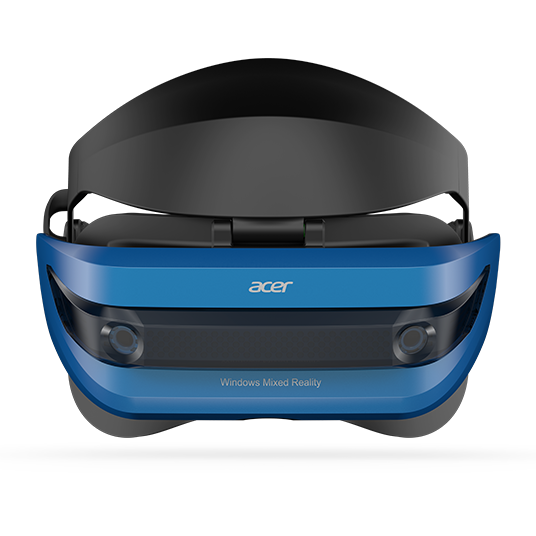
\includegraphics[scale=0.30]{Images/Estado del arte/acerh101.png}\\
        (a) Vista del casco completo
    \end{minipage}
    \begin{minipage}[t]{0.5\textwidth}
        \centering
        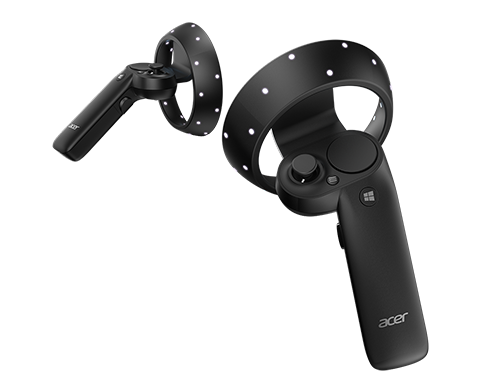
\includegraphics[scale=0.42]{Images/Estado del arte/acerh101controller.png}\\
       (b) Vista de los controladores
    \end{minipage}\\
    \caption[Dispositivo \textit{AcerAH101-D8EY}]{Dispositivo \textit{AcerAH101-D8EY}\footnotemark.}
    \label{fig:acerAH101}
\end{figure}

\footnotetext{Fuente: \href{https://www.acer.com/ac/en/US/content/model/VD.R05AP.002}{\nolinkurl{https://www.acer.com/model/VD.R05AP.002}}}

El campo de visión del casco es de 100\degree  y respecto a la resolución, es capaz de mostrar 2.880x1.440 píxeles combinando los dos ojos (1.440x1.440 píxeles en cada ojo), además, la distancia interpupilar no es ajustable y viene configurada por defecto a 62mm.\\



Por otro lado, ya que se conecta mediante \textit{bluetooth} necesita una fuente de energía de 2 pilas tipo AA, del mismo modo, el dispositivo viene con dos controladores que igualmente funcionan con 2 pilas del tipo AA cada uno y tienen 6 grados de libertad. \\

Los sensores que tiene este casco son: acelerómetro, giroscopio, magnetómetro y sensor de proximidad, además, el peso del dispositivo es de 848g. 